\documentclass[12pt,letterpaper]{article}
\usepackage{graphicx,textcomp}
\usepackage{natbib}
\usepackage{setspace}
\usepackage{fullpage}
\usepackage{color}
\usepackage[reqno]{amsmath}
\usepackage{amsthm}
\usepackage{fancyvrb}
\usepackage{amssymb,enumerate}
\usepackage[all]{xy}
\usepackage{endnotes}
\usepackage{lscape}
\newtheorem{com}{Comment}
\usepackage{float}
\usepackage{hyperref}
\newtheorem{lem} {Lemma}
\newtheorem{prop}{Proposition}
\newtheorem{thm}{Theorem}
\newtheorem{defn}{Definition}
\newtheorem{cor}{Corollary}
\newtheorem{obs}{Observation}
\usepackage[compact]{titlesec}
\usepackage{dcolumn}
\usepackage{tikz}
\usetikzlibrary{arrows}
\usepackage{multirow}
\usepackage{xcolor}
\newcolumntype{.}{D{.}{.}{-1}}
\newcolumntype{d}[1]{D{.}{.}{#1}}
\definecolor{light-gray}{gray}{0.65}
\usepackage{url}
\usepackage{listings}
\usepackage{color}

\definecolor{codegreen}{rgb}{0,0.6,0}
\definecolor{codegray}{rgb}{0.5,0.5,0.5}
\definecolor{codepurple}{rgb}{0.58,0,0.82}
\definecolor{backcolour}{rgb}{0.95,0.95,0.92}

\lstdefinestyle{mystyle}{
	backgroundcolor=\color{backcolour},   
	commentstyle=\color{codegreen},
	keywordstyle=\color{magenta},
	numberstyle=\tiny\color{codegray},
	stringstyle=\color{codepurple},
	basicstyle=\footnotesize,
	breakatwhitespace=false,         
	breaklines=true,                 
	captionpos=b,                    
	keepspaces=true,                 
	numbers=left,                    
	numbersep=5pt,                  
	showspaces=false,                
	showstringspaces=false,
	showtabs=false,                  
	tabsize=2
}
\lstset{style=mystyle}
\newcommand{\Sref}[1]{Section~\ref{#1}}
\newtheorem{hyp}{Hypothesis}

\title{Problem Set 1}
\date{Due: September 30, 2024}
\author{Athena Rodrigues}

\begin{document}
	\maketitle
	
	\section*{Instructions}
	\begin{itemize}
	\item Please show your work! You may lose points by simply writing in the answer. If the problem requires you to execute commands in \texttt{R}, please include the code you used to get your answers. Please also include the \texttt{.R} file that contains your code. If you are not sure if work needs to be shown for a particular problem, please ask.
\item Your homework should be submitted electronically on GitHub.
\item This problem set is due before 23:59 on Monday September 30, 2024. No late assignments will be accepted.
%\item Total available points for this homework is 80.
	\end{itemize}
	\section*{Question 1: Education}

A school counselor was curious about the average of IQ of the students in her school and took a random sample of 25 students' IQ scores. The following is the data set:\\
\lstinputlisting[language=R, firstline=36, lastline=36]{PS01_answersAR.R}  

\begin{enumerate}
	\item Find a 90\% confidence interval for the average student IQ in the school.\\
	
	\begin{Verbatim}
		90% CI = [94, 103]
	Code: 
	\end{Verbatim}
			\lstinputlisting[language=R, firstline= 39 , lastline=45] {PS01_answersAR.R}  
	\vspace{4cm}
	\item Next, the school counselor was curious  whether  the average student IQ in her school is higher than the average IQ score (100) among all the schools in the country.\\ 
	\noindent Using the same sample, conduct the appropriate hypothesis test with $\alpha=0.05$.
	\begin{Verbatim}
	Step 1: Assumptions
		The data y is a random, continous, numeric sample.
	Code:
	\end{Verbatim}
	\lstinputlisting[language=R, firstline= 54, lastline=55]{PS01_answersAR.R}  
	\begin{Verbatim}
	Step 2: Hypothesis
		The Null Hypothesis is that the mean is <= 100
		The Alternative Hypothesis is that the mean > 100
	Step 3: Calculate the Test Statistic
		The test statistic is -0.5957439.
	Code:
		\end{Verbatim}
		\lstinputlisting[language=R, firstline= 58, lastline=58]{PS01_answersAR.R}  
	\begin{Verbatim}
	Step 4: Calculate the P-Value
		The p-value is  0.7215383.
	Code:
	\end{Verbatim}
		\lstinputlisting[language=R, firstline=60, lastline=60]{PS01_answersAR.R}
	\begin{Verbatim}
	Step 5:
		Based on sufficient evidence, the p-value (0.7215) is 
		greater than the alpha (0.05),
		we fail to reject the null hypothesis that the 
		average IQ score is less than or equal to 100
	\end{Verbatim}
\end{enumerate}

\newpage

	\section*{Question 2: Political Economy}

\noindent Researchers are curious about what affects the amount of money communities spend on addressing homelessness. The following variables constitute our data set about social welfare expenditures in the USA. \\
\vspace{.5cm}


\begin{tabular}{r|l}
	\texttt{State} &\emph{50 states in US} \\
	\texttt{Y} & \emph{per capita expenditure on shelters/housing assistance in state}\\
	\texttt{X1} &\emph{per capita personal income in state} \\
	\texttt{X2} &  \emph{Number of residents per 100,000 that are "financially insecure" in state}\\
	\texttt{X3} &  \emph{Number of people per thousand residing in urban areas in state} \\
	\texttt{Region} &  \emph{1=Northeast, 2= North Central, 3= South, 4=West} \\
\end{tabular}

\vspace{.5cm}
\noindent Explore the \texttt{expenditure} data set and import data into \texttt{R}.
	\lstinputlisting[language=R, firstline = 68, lastline=69]{PS01_answersAR.R}
\vspace{.5cm}

\begin{itemize}

\item
Please plot the relationships among \emph{Y}, \emph{X1}, \emph{X2}, and \emph{X3}? What are the correlations among them (you just need to describe the graph and the relationships among them)?
\begin{figure}[h!]\centering
	\caption{\footnotesize Relationships Between Variables (Y, X1, X2, and X3)}
	\label{fig:plot_1}
	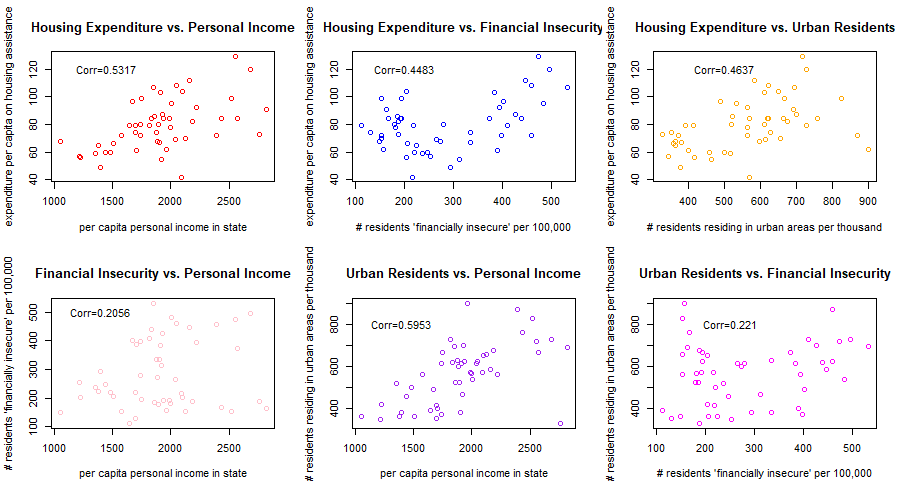
\includegraphics[width=.85\textwidth]{all_relationships.png}
\end{figure}
\vspace{1cm}
\begin{Verbatim}
Relationships:
Housing Expenditure vs. Personal Income (top left) shows 
a linear relationship with a strong, positive correlation. 
As personal income per capita in state increases 
so does the expenditure per capita on 
housing assistance in state.

Housing Expenditure vs. Financial Insecurity (top middle) has a
nonlinear relationship with a weak correlation.

Housing Expenditure vs. Urban Residents (top right) showcases a
linear relationship with a weak, positive correlation. 
This shows there is an effect in expenditure on 
housing assistance as urban areas grow.

Financial Insecurity vs. Personal Income (bottom left) has a
nonlinear relationship with little to no correlation. 
The variables of personal income and financial insecurity 
have little impact on eachother.

Urban Residents vs. Personal Income (bottom middle) has a linear relationship 
with a strong, positive correlation. There is a possible connection between 
increased personal income in state and increasing urban populations.

Urban Residents vs. Financial Insecurity (bottom right) has a nonlinear 
with little to no correlation. This shows that these 
variables have little impact in relation to each other.

 Code:
\end{Verbatim}
	\lstinputlisting[language=R, firstline= 81 , lastline=111] {PS01_answersAR.R}
\item
Please plot the relationship between \emph{Y} and \emph{Region}? On average, which region has the highest per capita expenditure on housing assistance?
\begin{figure}[h!]\centering
	\caption{\footnotesize Relationship between Y and Region}
	\label{fig:plot_2}
	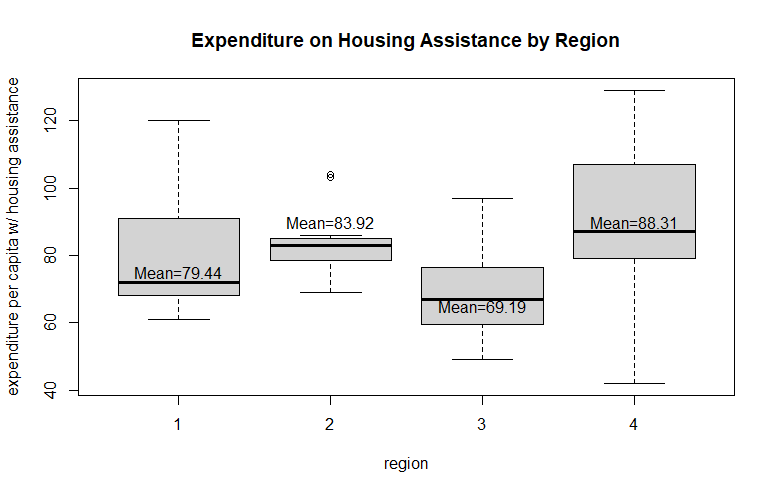
\includegraphics[width=.85\textwidth]{boxplot_yandregion.png}
\end{figure}
\begin{Verbatim}
	On average, the West (Region 4) has the highest per capita 
	expenditure on housing assistance at 88.31 followed by the
	North Central (Region 2), the Northeast (Region 1), 
	and the South (Region 3).
	
	Code:
\end{Verbatim}
	\lstinputlisting[language=R, firstline= 116 , lastline=123] {PS01_answersAR.R}
\item
Please plot the relationship between \emph{Y} and \emph{X1}? Describe this graph and the relationship. Reproduce the above graph including one more variable \emph{Region} and display different regions with different types of symbols and colors.
 \begin{Verbatim}
	Region 1 and 3 have a positive linear relationship and
	a wide data spread with strong correlations.
	Region 2 and 4 have a nonlinear relationship with a central 
	distribution of data and little to no correlation between variables.
	This means, according to these basic correlation tests,
	that states in the Northeast and the South generally see
	an increase in expenditure per capita on housing assistance 
	when personal income per capita increases as well, 
	however, this cannot be said for the North Central and West.
	
	Code:
 \end{Verbatim}
	\lstinputlisting[language=R, firstline= 128 , lastline= 140] {PS01_answersAR.R}
\begin{figure}[h!]\centering
		\caption{\footnotesize Relationship between Y and X1 based on Region}
		\label{fig:plot_3}
		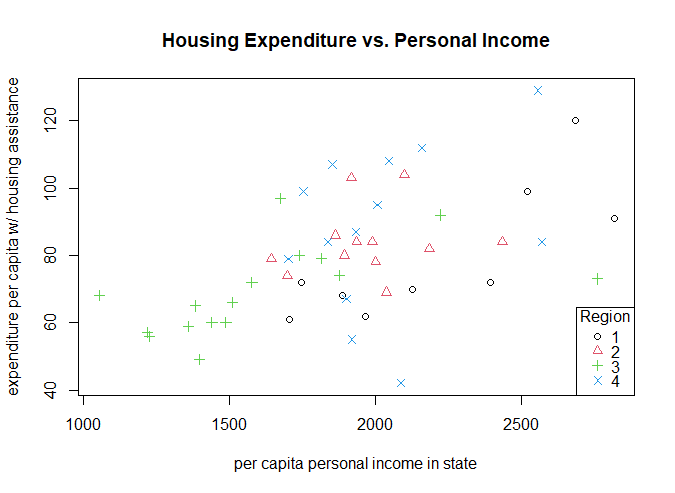
\includegraphics[width=.85\textwidth]{yx1_byregion.png}
\end{figure}
\end{itemize}

\end{document}
